%/*
% * SPDX-FileCopyrightText: 2021 Stefan Begerad <stefan@begerad.de>
% *
% * SPDX-License-Identifier: GPL-3.0-or-later
% */

\begin{frame}{Übersicht der IT-Infrastruktur}
  %alternative alignment to center is left and right
  \begin{center}
    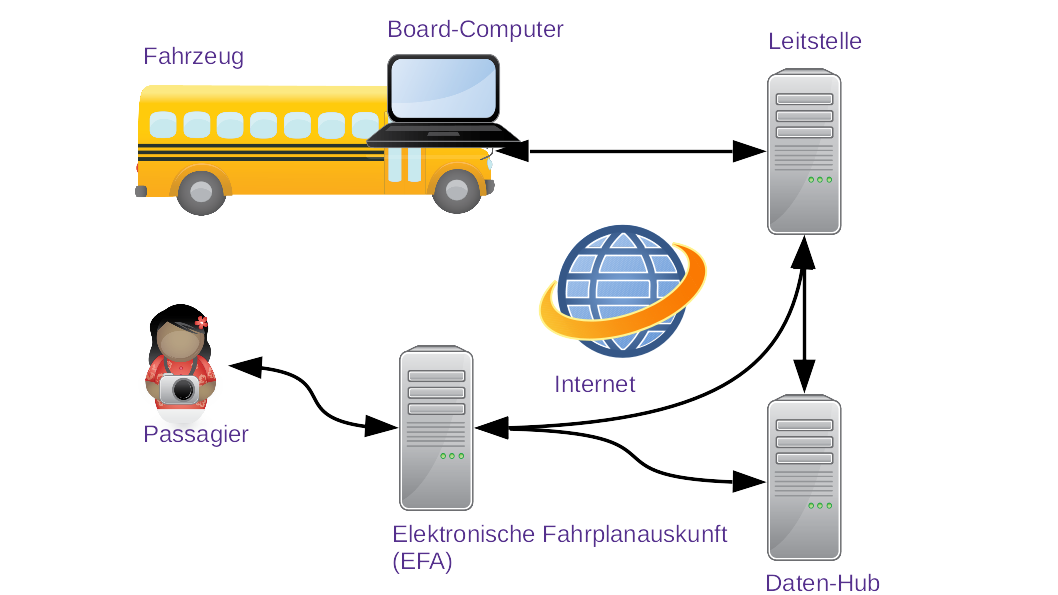
\includegraphics[width=1.1\textwidth]{otm-june-2-2021/public-transport-05-04-2021.png}
  \end{center}
\end{frame}

\begin{frame}{Board-Computer für Fahrzeuge}
  %alternative alignment to center is left and right
  
\includegraphics[width=0.2\textwidth]{otm-june-2-2021/bus.png}
  \begin{itemize}
  \item Investitionskosten pro Fahrzeug: etwa 2 bis 3 Tausend Euro
  \item Betriebskosten:
    \begin{itemize}
    \item Lizenskosten
    \item Supportkosten
    \end{itemize}
  \item Interaktion mit
    \begin{itemize}
    \item Fahrzeugnetzwerk bspw. IBIS,
    \item Ticket-Drucker oder -Scanner,
    \item Anzeige für Fahrdienst,
    \item Leitstelle per Analog- (Kurzwelle) oder Digitalfunk (Mobilfunk)
    \item Ortung per GPS
    \end{itemize}
  \end{itemize}
\end{frame}

